     %%%%%%%%%%%%%%%%%%%%
     %                  %
     %  capitolo6.tex   %
     %                  %
     %%%%%%%%%%%%%%%%%%%%

\chapter{Combinazione di misure dell'angolo $\gamma$}
\noindent
In questo capitolo si illustreranno i tre principali metodi impiegati per la valutazione di $\gamma$, chiamati \emph{GLW} (Gronau-London-Wyler, \cite{Gronau:1990ra}\cite{Gronau:1991dp}), 
\emph{ADS} (Atwood-Dunietz-Soni, \cite{Atwood:1996ci}) e \emph{GGSZ} (Giri-Grossman-Soffer-Zupan, \cite{Giri:2003ty}) 
\begin{figure}
\begin{center}
\includegraphics[scale=0.3]{Immagini/diagrammi}
\caption{Decadimenti $B^{-} \longrightarrow D[\rightarrow f]K^{-}$ studiati per misurare il valore dell'angolo $\gamma$}
\label{DIAGRAMMIDIFEYNMAN}
\end{center}
\end{figure}

La misura di $\gamma$ si basa sullo studio delle interferenze dei decadimenti $b\rightarrow u$ e $b\rightarrow c$ in processi ad albero del tipo:
\begin{equation}\label{B-dec}
 B^{-} \longrightarrow D[\rightarrow f]K^{-}
\end{equation}
nei quali $D$ può indicare sia il $D^0$ che a il $\bar{D^0}$ (Fig. \ref{DIAGRAMMIDIFEYNMAN}). 
Le interferenze tra le diverse ampiezze di decadimento dipendono dalla fase debole $\gamma$.

I tre metodi menzionati differiscono tra loro per i diversi stati finali di $D$  usati nell'analisi:
\begin{enumerate}
 \item \emph{GLW}: analizza i decadimenti nei quali gli stati finali del $D$ sono CP-coniugati (ad esempio $D\rightarrow \pi\pi$).
 \item \emph{ADS}: si basa sui decadimenti \emph{Cabibbo favoriti} (CF) (ad esempio $B^-\rightarrow D^0[\rightarrow K^{-}\pi^{+}] K^-$) e \emph{doppiamente Cabibbo soppressi} (DCS) (ad esempio $B^-\rightarrow D[\rightarrow K^{+}\pi^{-}] K^-$).
 \item \emph{GGSZ}:analizza i decadimenti C-coniugati in tre corpi (ad esempio $D\rightarrow K_S K^\pm K^\mp$). 
                   Per misuare le osservabili dipendenti da $\gamma$ è necessario eseguire un'analisi di Dalitz.
\end{enumerate}
La migliore precisione su $\gamma$ si ottiene combinando i risultati di tutte queste analisi. 

Di seguito sono definiti alcuni parametri che risulteranno utili nella trattazione successiva:
\begin{enumerate}
 \item $r$: rapporto fra le ampiezze di decadimento DCS e CF del $B$ e del $D$;
 \item $\delta$: differenza di fase forte;
 \item Le ampiezze di decadimento del $B^-$ e del $D$ possono essere scritte nel seguente modo:
\begin{displaymath}
\left\{
\begin{array}{l}
A(B^- \rightarrow DK^-) = A_ce^{i\delta_c}\\
A(B^- \rightarrow \bar{D}K^-) = A_ue^{i\delta_u-\gamma}\\
A(D \rightarrow f) = A_fe^{i\delta_f}\\
A(D \rightarrow \bar{f}) = A_ce^{i\delta_{\bar{f}}}
\end{array}
\right.
\end{displaymath}
dove $A_c$, $A_u$, $A_f$ e $A_{\bar{f}}$ sono grandezze reali e positive. Si è ignorata la violazione di CP nel decadimento del $D$ (si noti l'assenza del termine $\gamma$
nei decadimenti di quest'ultimo). Gli indici $u$ e $c$ si riferiscono rispettivamente alle transizioni $b\rightarrow u$ e $b\rightarrow c$.
Qualora il $D^0$ segua un canale di decadimento in tre corpi, le quantità $A_f$, $A_{\bar{f}}$, $\delta_f$ e $\delta_{\bar{f}}$ saranno funzioni delle coordinate nel diagramma
di Dalitz.
\end{enumerate} 
L'ampiezza del decadimento $B^- \rightarrow D[\rightarrow f]K^-)$ è data dall'equazione:
\begin{equation}
 A (B^-\rightarrow D[\rightarrow f]K^-) = A_cA_fe^{i(\delta_c + \delta_f)} + A_u A_fe^{i\delta_u + \delta_{\bar{f}} - \gamma}
\end{equation}
Da cui si deduce la seguente espressione per il tasso di decadimento:
\begin{equation}\label{probability}
 \Gamma (B^-\rightarrow D[\rightarrow f]K^-) \propto A_c^2\big(A_f^2 + r_B^2A_{\bar{f}}^2 + 2r_BA_fA_{\bar{f}}\cos(\delta_B + \delta_D - \gamma)\big)
\end{equation}
con $r_B = A_u/A_c$, $\delta_B = \delta_u - \delta_c$ e $\delta_D = \delta_{\bar{f}} - \delta_f$.

Nei paragrafi successivi verrà descritta l'analisi che permette di combinare le recenti misure di LHCb nei decadimento $B^{\pm}\rightarrow DK^{\pm}$ 
\cite{LHCBB2}\cite{LHCBB3}\cite{LHCBB4} per estrarre, 
mediante un metodo basato sulla statistica di Bayes, gli intervalli di credibilità dell'angolo $\gamma$ e dei parametri di interesse associati. Le analisi sono 
realizzate con i dati raccolti da LHCb nel 2011, corrispondenti ad una luminosità integrata di $1$ $fb^{-1}$, nelle collisioni $p$-$p$ ad LHC.  Nei seguenti paragrafi,
verranno brevemente descritti i metodi GLW, ADS e GGSZ, il metodo di estrazione di gamma mediante la statistica bayesiana ed infine verranno discussi i risultati. 


\section{Metodo GLW}
\noindent
Nell'analisi GLW, si studiano decadimenti ad albero i cui prodotti finali sono autostati di CP, ad esempio:
\begin{equation}
 D\longrightarrow K^-K^+\ \ \ \ \ \ \ \ \ \ \ \ \ \ \ \ (CP = +1)
\end{equation}
\begin{equation}
 D\longrightarrow K_s\pi^0\ \ \ \ \ \ \ \ \ \ \ \ \ \ \ \ \ \ (CP = -1)
\end{equation}
Per cui si ha ${A_f}/A_{\bar{f}} = 1$ e $\delta_D = 0, \pi$. Pertanto l'equazione \eqref{probability} diventa:
\begin{equation}\label{numera}
 \Gamma(B^- \rightarrow D^0[\rightarrow f_{CP=\pm1}]K^-) \propto A_c^2 (1 + r_B^2 \pm 2r_B\cos(\delta_B - \gamma))
\end{equation}
Per normalizzare questa espressione possono essere usati i decadimenti ad albero $B^-\rightarrow D^0[\rightarrow K^{-}\pi^{+}] K^-$ e $B^-\rightarrow \bar{D^0}[\rightarrow K^{+}\pi^{-}] K^-$ 
, nei quali cioè il $D^0$ decade secondo i canali CF. Si può scrivere, con buona approssimazione:
\begin{equation}\label{normalizzazione}
 \Gamma(B^-\rightarrow D^0[\rightarrow K^-\pi^+]K^-) =  \Gamma(B^-\rightarrow \bar{D}^0[\rightarrow K^+\pi^-]K^-) = \propto A_c^2
\end{equation}
A questo punto è possibile definire gli osservabili $R_{CP\pm}$ e $A_{CP\pm}$ nel modo seguente:
\begin{equation}\label{RCP}
 R_{CP\pm} = \frac{2[\Gamma(B^- \rightarrow D_{CP\pm}^0K^-) + \Gamma(B^+\rightarrow D_{CP\pm}^0K^+)]}{\Gamma (B^-\rightarrow D^0K^-) + \Gamma (B^+ \rightarrow \bar{D}^0K^+)} = 1 + r_B^2 \pm 2r_B \cos \delta_B \cos \gamma
\end{equation}
\begin{equation}\label{ACP}
 A_{CP\pm} = \frac{\Gamma(B^- \rightarrow D_{CP\pm}^0K^-) - \Gamma(B^+\rightarrow D_{CP\pm}^0K^+)}{\Gamma(B^- \rightarrow D_{CP\pm}^0K^-) + \Gamma(B^+\rightarrow D_{CP\pm}^0K^+)} = \frac{\pm 2r_B\sin\delta_B\sin\gamma}{R_{CP\pm}}
\end{equation}
Le due equazioni \eqref{RCP} e \eqref{ACP} forniscono un sistema di quattro equazioni nelle tre incognite $\gamma$, $r_B$ e $\delta_B$, 
quindi una misura di $R_{CP\pm}$ e di $A_{CP\pm}$ permette di ottenere una misura di queste tre quantità. 
Lo stato sperimentale di queste misure è riportato in Tab. \ref{tab:Acp}.

\begin{table}
  \begin{center}
    \begin{small}
      \begin{tabular}{|c|c|c|c|c|}

\hline
 & \textbf{$A_{CP+}$} & \textbf{$A_{CP-}$} & \textbf{$R_{CP+}$} & \textbf{$R_{CP-}$}\\
\hline
\textbf{BaBar} & $0.25 \pm 0.06 \pm 0.02$ & $-0.09 \pm 0.07 \pm 0.02$  & $1.18 \pm 0.09 \pm 0.05$ & $1.07 \pm 0.08 \pm 0.04$\\
\hline
\textbf{Belle} & $0.29 \pm 0.06 \pm 0.02$ & $-0.12 \pm 0.06 \pm 0.01$ & $1.03 \pm 0.07 \pm 0.03$& $1.13 \pm 0.09 \pm 0.05$\\
\hline
\textbf{CDF} & $0.39 \pm 0.17 \pm 0.04$ & - & $1.30 \pm 0.24 \pm 0.12$ & -\\
\hline
\textbf{LHCb} & $0.14 \pm 0.03 \pm 0.01$ & - & $1.01 \pm 0.04 \pm 0.01$ & -\\
\hline
\textbf{Media} & $0.19 \pm 0.03$ & $-0.11 \pm 0.05$ & $1.03 \pm 0.03$ & $1.10 \pm 0.07$\\
\hline
      \end{tabular}
    \end{small}
  \end{center}
\caption{Stato sperimentale attuale (2012) delle misure dei parametri $A_{CP+}$, $A_{CP-}$, $R_{CP+}$ e $R_{CP-}$. I valori medi sono quelli ottenuti dalla collaborazione
         HFAG\cite{HFAG}.}
\label{tab:Acp}

\end{table}


\section{Metodo ADS}
\noindent
Nell'analisi ADS, vengono selezionati i canali di decadimento CF (ad esempio $B\rightarrow D^0[\rightarrow K^{-}\pi^{+}] K^-$) e 
DCS (ad esempio $B\rightarrow D^0[\rightarrow K^{+}\pi^{-}] K^-$).

Il tasso di decadimento sensibile a $\gamma$ è il risultato dell'interferenza del canale favorito dal punto di vista del colore $B^-\rightarrow D^0K^-$ seguito dal processo
doppiamente Cabibbo soppresso $D^0\rightarrow \pi^-K^+$ e dal canale sfavorito da punto di vista del colore $B^-\rightarrow \bar{D^0}K^-$ seguito dal canale
Cabibbo favorito $D^0\rightarrow K^-\pi^+$. Le ampiezze in gioco sono di grandezza simile, per cui gli effetti di interferenza tra le due sono di notevole intensità.
A partire dall'equazione \eqref{probability} si dimostra che:
\begin{equation} \label{GLWgamma}
 \Gamma(B^{\mp}\rightarrow D^0[\rightarrow K^{\pm}\pi^{\mp}]K^{\mp}) \propto r_B^2 + r_D^2 \pm 2r_Br_D \cos(\delta_B + \delta_D \mp \gamma)
\end{equation}
dove $r_B = A_f/A_{\bar{f}} = |A(D^0 \rightarrow \pi^-K^+)/A(D^0\rightarrow K^-\pi^+)|$ e $\delta_D$ è la differenza di fase forte tra i due decadimenti. $r_D$ e $\delta_D$
entrano nell'analisi come parametri noti, il cui valore può essere determinato usando i dati raccolti dalla collaborazione Cleo nelle collisioni elettrone-positrone alla 
risonanza $\psi(3770)$ \cite{cleo}. È possibile ora definire le quantità $R_{ADS}$ e $A_{ADS}$:
\begin{equation}
 R_{ADS} = \frac{\Gamma(B^- \rightarrow D^0[\rightarrow \pi^- K^+]K^-) + \Gamma(B^+ \rightarrow D^0[\rightarrow \pi^+K^-]K^+)}{\Gamma(B^- \rightarrow D^0[\rightarrow K^- \pi^+]K^-) + \Gamma(B^+ \rightarrow D^0[\rightarrow K^+\pi^-]K^+)}
\end{equation}
\begin{equation}
 A_{ADS} = \frac{\Gamma(B^- \rightarrow D^0[\rightarrow \pi^- K^+]K^-) - \Gamma(B^+ \rightarrow D^0[\rightarrow \pi^+K^-]K^+)}{\Gamma(B^- \rightarrow D^0[\rightarrow K^- \pi^+]K^-) + \Gamma(B^+ \rightarrow D^0[\rightarrow \pi^+K^-]K^+)}
\end{equation}
Sostituendo in queste espressioni le equazioni \eqref{normalizzazione} e \eqref{GLWgamma} si ottiene:
\begin{equation}
 R_{ADS} = r_B^2 + r_{K\pi}^2 + 2r_Br_{K\pi}\cos\gamma\cos(\delta_B + \delta_{D})
\end{equation}
\begin{equation}
 A_{ADS} = \frac {2r_B r_{K\pi}\sin\gamma\sin(\delta_B + \delta_{D})}{R_{ADS}}
\end{equation}
Queste due quantità hanno lo svantaggio di essere correlate. È possibile definire le due variabili scorrelate $R_\pm$:
\begin{equation}
 R_{\pm} = \frac{\Gamma(B^{\pm}\rightarrow D^0[\rightarrow K^{\mp}\pi^{\pm})]K^{\mp})}{\Gamma(B^{\pm}\rightarrow D^0[\rightarrow K^{\pm}\pi^{\mp}]K^{\pm})} = \frac{1}{N}(r_B^2 + r_{K\pi}^2 + 2r_Br_{K\pi}\cos(\delta_B + \delta_{K\pi} \pm \gamma)) 
\end{equation}
dove $N$ è una costante vicina ad uno. Queste due nuove quantità sono statisticamente indipendenti.
\begin{table}
\begin{center}
\begin{tabular}{|c|c|c|}\hline
 & \textbf{$A_{ADS}$} & \textbf{$R_{ADS}$}\\\hline
\textbf{BaBar} & $-0.86 \pm 0.47_{-0.16}^{+0.12}$ & $0.011 \pm 0.006 \pm 0.002$\\\hline
\textbf{Belle} & $-0.39_{-0.28 -0.03}^{+0.26 +0.04}$ & $0.0163_{- 0.0041 - 0.0013}^{+0.0044 + 0.0007}$\\\hline
\textbf{CDF} & $-0.82 \pm 0.44 \pm 0.09$ & $0.0220 \pm 0.0086 \pm 0.0026$\\\hline
\textbf{LHCb} & $-0.52 \pm 0.15 \pm 0.02$ & $0.0152 \pm 0.0020 \pm 0.0004$\\\hline
\textbf{Media} & $-0.54 \pm 0.12$ & $0.0153 \pm 0.0017$\\\hline
\end{tabular}
\end{center}
\caption{Stato attuale (2012) delle misure sperimentali di $A_{ADS}$ e $R_{ADS}$. I valori medi sono quelli ottenuti dalla collaborazione
         HFAG\cite{HFAG}.}
\label{referenzatabella}
\end{table}
Lo stato sperimentale delle grandezze $A_{ADS}$ e $R_{ADS}$ è riportato in Tab. \ref{referenzatabella}. 


\section{Metodo GGSZ}
\noindent
Nell'analisi GGSZ, vengono studiati i decadimenti in tre corpi C-coniugati del $D$:
\begin{equation}\label{decadimento}
 D \rightarrow K_S\pi^+\pi^- \ \ \ \ \ \ \ \ \ \ \ \ \ \ \ \ D \rightarrow K_SK^+K^-
\end{equation}
Le ampiezze sono $A_fe^{i\delta_f} = f(m_-^2, m_+^2)$ e $A_{\bar{f}}e^{i\delta_{\bar{f}}} = f(m_+^2, m_-^2)$
dove si è indicata con $m_+$ la massa del sistema $K_S\pi^+(K^+)$ e con $m_-$ quella di $K_S\pi^-(K^-)$.
I tassi di decadimento possono essere scritti come:
\begin{equation}\label{GGSZ}
 \Gamma(B^{\mp} \rightarrow D[\rightarrow K_Sh^+h^-)]K^{\mp}) \propto  
\end{equation}
\begin{equation*}
 \propto |f(m_{\mp}^2, m_{\pm}^2)|^2 + r_B^2|f(m_{\pm}^2, m_{\mp}^2)|^2 + 2r_B|f(m_{\mp}^2 + m_{\pm}^2)||f(m_{\mp}^2, m_{\pm}^2)\cos(\delta_B + \delta_D(m_{\mp}^2, m_{\pm}^2)\mp \gamma)
\end{equation*}
dove $h$ può indicare un $\pi$ o un $K$, mentre $\delta_D(m_{\mp}^2, m_{\pm}^2)$ è la differenza di fase forte tra $f(m_{\pm}^2, m_{\mp}^2)$ e $f(m_{\mp}^2, m_{\pm}^2)$.

Introducendo le \emph{coordinate cartesiane}, definite come:
\begin{equation}
 x_{\pm} = \Re [r_Be^{i(\delta_B \pm \gamma)}]
\end{equation}
\begin{equation}
 y_{\pm} = \Im [r_Be^{i(\delta_B \pm \gamma)}]
\end{equation}
è possibile riscrivere la \eqref{GGSZ} come:
\begin{equation}
\Gamma(B^{\mp} \rightarrow D^0[\rightarrow K_S\pi^+\pi^-)]K^{\mp}) \propto |f_{\mp}|^2 + r_B^2|f_{\pm}|^2 + 2[x_{\mp}\Re[f_{\mp}f_{\pm^*}] + y_{\mp} \Im[f_{\mp}f_{\pm}]] 
\end{equation}
dove sono state usate le notazioni compatte $f_{\pm} = f(m_{\pm}^2, m_{\mp}^2)$ e $f_{\mp} = f(m_{\mp}^2, m_{\pm}^2)$.
\begin{table}
\begin{center}
\footnotesize
\begin{tabular}{|c|c|c|c|c|}\hline
 & \textbf{BaBar} & \textbf{Belle} & \textbf{Media} & \textbf{LHCb}\\\hline
$x_+$ & $-0.103\pm0.037\pm0.006\pm0.007$ & $-0.107\pm0.043\pm0.011\pm0.055$ & $-0.104\pm0.029$ & $-0.1030 \pm 0.0504$\\\hline
$y_+$ & $-0.021\pm0.048\pm0.004\pm0.009$ & $-0.067\pm0.059\pm0.018\pm0.063$ & $0.085\pm0.030$ & $-0.009 \pm0.048$\\\hline
$x_-$ & $0.060\pm0.039\pm0.007\pm0.006$ & $0.105\pm0.047\pm0.018\pm0.063$ & $0.085\pm0.030$ & $0.000 \pm0.0459$ \\\hline
$y_-$ & $0.062\pm0.045\pm0.004\pm0.006$ & $0.177\pm0.060\pm0.018\pm0.054$ & $0.105\pm0.036$ & $0.0270 \pm 0.0574$\\\hline
\end{tabular}
\normalsize
\end{center}
\caption{Stato attuale (2012) delle misure dei parametri $x_\pm$ e $y_\pm$. I valori medi sono quelli ottenuti dalla collaborazione
         HFAG\cite{HFAG}.}
\label{xy}
\end{table}
I valori sperimentali di $x_\pm$ e $y_\pm$ sono riportati in Tab. \ref{xy}.

\section{Statistica Bayesiana}
\noindent
Nei paragrafi precedenti è stato descritto come sia possibile misurare, attraverso lo studio dei decadimenti $B^\pm \rightarrow D^0K^\pm$,
alcune osservabili che sono funzioni dell'angolo $\gamma$. Per combinare tutte le osservabili ed ottenere un'unica misura di $\gamma$ sarà usata l'\emph{analisi statistica 
bayesiana}.
Di seguito è riportato l'enunciato teorema di Bayes, con una semplice dimostrazione.

\begin{teorema}
 Si consideri un gruppo completo di ipotesi incompatibili, dette $H_1$, $H_2$, $...$ , $H_n$. Si esegue ora un esperimento che porta al verificarsi dell'evento $A$.
Allora, la probabilità che $A$ sia stato causato dalla validità dell'ipotesi $H_i$ è data da:
\begin{equation}
 P(H_i|A) = \frac{P(H_i)P(A|H_i)}{\sum_{i = 1}^n P(H_i)P(A|H_i)}
\end{equation}
\end{teorema}
\begin{proof}
 In accordo con la regola di moltiplicazione delle probabilità si ha:
\begin{equation}
 P(AH_i) = P(A|H_i)P(H_i) = P(H_i|A)P(A)
\end{equation}
Risolvendo rispetto a $P(H_i|A)$ si ottiene:
\begin{equation}\label{PHiA}
P(H_i|A) = \frac{P(H_i)P(A|H_i)}{P(A)}
\end{equation}
Ma la probabilità che si verifichi $A$ è data dalla somma sulle $n$ ipotesi $H_n$ dei prodotti $P(A|H_i)P(H_i)$:
\begin{equation}\label{PA}
P(A) = \sum_{i = 1}^n P(H_i)P(A|H_i) 
\end{equation}
Per cui, sostituendo la \eqref{PA} nella \eqref{PHiA} si ottiene la tesi.
\end{proof}
L'ovvia generalizzazione al caso continuo di quanto esposto è:
\begin{equation}
 f(H|A) = \frac{f(H)f(A|H)}{\int f(H)f(A|H)dH}
\end{equation}
Le grandezze che compaiono in questa formula non sono più probabilità discrete ma densità di probabilità \cite{d'agostini}. Esse sono definite nel modo seguente:
\begin{enumerate}
 \item $f(A|H)$, cioè la probabilità di registrare un certo valore sperimentale $A$ data l'ipotesi $H$, è detta anche \emph{verosimiglianza}
 \item $f(H)$, cioè la probabilità di validità dell'ipotesi $H$, detta anche probabilità \emph{a priori} o \emph{prior}. In mancanza di informazioni ulteriori che rendano alcune 
       ipotesi più probabili di altre viene si assume che abbia lo stesso valore su ogni $H$. 
 \item $f(H|A)$, cioè la probabilità di validità dell'ipotesi $H$ una volta registrato il dato sperimentale $A$. Viene anche detta probabilità \emph{a posteriori}.
\end{enumerate}
Nel caso più generale $H$ ed $A$ sono grandezze vettoriali:
\begin{equation}
  f(\vec{H}|\vec{A}) = \frac{f(\vec{H})f(\vec{A}|\vec{H})}{\int f(\vec{H})f(\vec{A}|\vec{H})d\vec{H}}
\end{equation}
Nell'analisi svolta in questa tesi si ha:
\begin{enumerate}
 \item $\vec{H} = (\gamma, r_B, \delta_B, r_D, \delta_D)$
 \item $\vec{A} = (R_{CP+}, A_{CP+}, R_+, R_-, x_\pm, y_\pm)$
\end{enumerate}
Per ottenere la misura di $\gamma$ è necessario conoscere la densità di probabilità \emph{a posteriori} $f(\vec{H}|\vec{A})$ in maniera da ottenere da questa la densità
di probabilità di $\gamma$, $f(\gamma)$, secondo la formula:
\begin{equation}
 f(\gamma) = \int f(\vec{H}|\vec{A}) dr_Bd\delta_Bdr_Dd\delta_D
\end{equation}
Uno strumento di calcolo utile a questo scopo è il \emph{framework} BAT, che verrà descritto nel seguente paragrafo.

\section{BAT (\emph{Bayesian Analysis Toolkit})}
\noindent
Per determinare la distribuzione di probabilità \emph{a posteriori} $f(\vec{H}|\vec{A})$ si è utilizzato il \emph{framework} BAT.
Esso implementa alcuni algoritmi utili a realizzare l'analisi bayesiana dei dati.
Lo scopo  è quello di dare risposta a due esigenze:
\begin{enumerate}
 \item fornire uno strumento flessibile che permetta la formulazione di ogni tipo di modello
 \item fornire un codice di analisi numerica fortemente ottimizzato che permetta la gestione di una grande quantità di operazioni
\end{enumerate}
È scritto in C++ e si basa su ROOT per le funzioni di input/output e realizzazione di grafici.
Le sue funzioni includono la mappatura della probabilità a posteriori in uno spazio dei parametri multidimensionale,
la stima dei parametri e dei relativi intervalli di credibilità, il calcolo della correlazione tra diversi parametri, etc.
Il cuore centrale di BAT è costituito da \emph{Metropolis}, un algoritmo che implementa il metodo MCMC (\emph{Markov Chain Monte Carlo}) e che verrà discusso dettagliatamente nel seguito.
\subsection{Markov Chain Monte Carlo}
\noindent
Ottenere la probabilità \emph{a posteriori} è solitamente un problema molto difficile, specialmente nel caso di un modello con un alto numero di parametri.
In particolare, risulta particolarmente dispendioso dal punto di vista del calcolo trovare il fattore di normalizzazione $\int f(\vec{H})f(\vec{A}|\vec{H})d\vec{H}$.
Per ovviare a questa difficoltà vengono largamente impiegati metodi numerici, in modo particolare il metodo MCMC, che permette di estrarre numeri casuali secondo 
la distribuzione statistica $f(\vec{H})f(\vec{A}|\vec{H})/\int f(\vec{H})f(\vec{A}|\vec{H})d\vec{H}$ senza conoscere il fattore di 
normalizzazione $\int f(\vec{H})f(\vec{A}|\vec{H})d\vec{H}$, cioè ammettendo come unica ipotesi di poter confrontare la distribuzione in due punti arbitrari 
$\vec{H_i}$ ed $\vec{H_j}$ calcolando il rapporto $\frac{f(\vec{H_i})f(\vec{A}|\vec{H_i})}{f(\vec{H_j})f(\vec{A}|\vec{H_j})}$.
 
Come indica il nome, si tratta di un processo di Markov, per cui ogni valore $f(\vec{H_i})f(\vec{A}|\vec{H_i})$ calcolato con questa tecnica risulta correlato 
al precedente $f(\vec{H_{i-1}})f(\vec{A}|\vec{H_{i-1}})$ ed indipendente da tutti gli altri.
L'algoritmo che lo implementa all'interno di BAT, \emph{Metropolis}, consta di quattro passi:
\begin{enumerate}
 \item Si sceglie un punto $\vec{H_i}$ nello spazio dei parametri, la cui dimensionalità dipenderà dal tipo di problema studiato
 \item Si sceglie in maniera casuale un secondo punto $H'$, usando una distribuzione statistica a simmetria sferica centrata in $H_i$, 
       $g_{H_i}(H_i')$ (solitamente si tratta di una distribuzione uniforme in un dato intorno di $H_i$ e nulla al di fuori).
 \item Si calcolano $f(\vec{H_i})f(\vec{A}|\vec{H_i})$ e $f(\vec{H'})f(\vec{A}|\vec{H'})$.
       Se $f(\vec{H'})f(\vec{A}|\vec{H'}) \geq f(\vec{H_i})f(\vec{A}|\vec{H_i})$ si pone $H_{i+1} = H'$. 
       Se $f(\vec{H'})f(\vec{A}|\vec{H'}) \leq f(\vec{H_i})f(\vec{A}|\vec{H_i})$ il valore di $H_{i+1}$ verrà scelto in maniera aleatoria:
       si avrà $H_{i+1} = H'$ con probabilità pari a $\frac{f(\vec{H'})f(\vec{A}|\vec{H'})}{f(\vec{H_i})f(\vec{A}|\vec{H_i})}$, altrimenti $H_{i+1} = H_i$ (con, ovviamente, probabilità pari a $1-\frac{f(\vec{H'})f(\vec{A}|\vec{H'})}{f(\vec{H_i})f(\vec{A}|\vec{H_i})}$).
 \item A questo punto il ciclo viene iterato a partire dal secondo passo.
\end{enumerate}
È ragionevole supporre che, dopo un certo numero di cicli, l'istogramma normalizzato delle $H_i$ campionate darà un'approssimazione sufficientemente accurata della 
distribuzione $f(\vec{H}|\vec{A})$. Si può anche procedere in maniera formale e dimostrare che la catena di Markov impiegata nel procedimento ammette come 
distribuzione di equilibrio la funzione $f(\vec{H}|\vec{A})$ ricercata, ma la discussione è al di là del livello di questa tesi, per cui non verrà qui affrontata.

\section{Osservabili e metodo di misura}
\noindent
Come già accennato la misura di $\gamma$ verrà effettuata calcolando grazie a BAT la seguente densità di probabilità:
\begin{equation}
   f(\vec{H}|\vec{A}) = \frac{f(\vec{H})f\vec{A}|\vec{H})}{\int f(\vec{H})f(\vec{A}|\vec{H})d\vec{H}}
\end{equation}
Dove $f(\vec{H})$ è la distribuzione statistica \emph{a priori}, data dal prodotto delle cinque distribuzioni \emph{a priori} delle incognite del problema ($\gamma$, $r_B$, $\delta_B$, $r_D$ e $\delta_D$).
Poiché la combinazione eseguita vuole essere indipendente dalle misure precedenti di $\gamma$, $r_B$ e $\delta_B$;
le distribuzioni \emph{a priori} di queste grandezze vengono poste costanti.
Per $r_D$ e $\delta_D$, al contrario, si scelgono come \emph{prior} delle gaussiane centrate sui valori 
delle due grandezze forniti dalla collaborazione Cleo e di deviazione standard pari all'incertezza sperimentale sugli stessi.
Infatti il sistema non ha sensibilità sufficiente a gestire una distribuzione piatta anche su queste grandezze per cui, se non si inserisse su queste un'informazione
esterna (cioè la misura di Cleo), ne risulterebbe un valore di $\gamma$ completamente indeterminato.

\begin{table}
\begin{center}
\begin{tabular}{|c|c|}
\hline
\textbf{Osservabile} & \textbf{Distribuzione a priori}\\\hline
$\gamma$ & $\chi[0 , 180]$\\\hline
$\delta_B$ & $\chi[0,180]$\\\hline
$r_B$ & $\chi[0, 0.3]$\\\hline
$\delta_D$ & $G(-152, 10)$\\\hline
$r_D$ & $G(0.00376, 0.00009)$\\\hline
\end{tabular}
\end{center}
\caption{Si è indicata con $\chi[a,b]$, $a,b \in \mathbb{R}$ la funzione caratteristica dell'intervallo $[a,b]$ (normalizzata in maniera tale da avere integrale unitario sul dominio), 
mentre con $G(\bar{x}, \sigma)$ ($\bar{x}, \sigma \in \mathbb{R}$) si è indicata la funzione di Gauss (anch'essa normalizzata ad uno) di media $\bar{x}$ e deviazione standard $\sigma$.}
\label{tabellaprior}
\end{table}
I cinque \emph{prior} sono elencati brevemente in Tab. \ref{tabellaprior}.
La verosimiglienza $f(\vec{A}|\vec{H})$ è data dalla formula seguente:
\begin{equation}
 f(\vec{A}|\vec{H}) = \prod_i \exp-\left(\frac{(A_i(\vec{H}) - O_i)^2}{2\sigma_{O_i}}\right)
\end{equation}
dove con $O_i$ è stato indicato il valore misurato dell'$i$-esimo osservabile, con $\sigma_{O_i}$ la sua incertezza e con $c_i(\alpha)$ la sua espressione come funzione delle
incognite, ricavata attraverso i tre metodi GLW, ADS e GGSZ discussi in precedenza.
In Tab.\ref{O_i} sono riportati i valori $O_i$ e $\sigma_{O_i}$ relativi a ciascuna osservabile, nonché l'espressione della stessa in funzione delle incognite. 
\begin{table}
\begin{center}
\begin{tabular}{|c|c|c|c|}\hline
\textbf{Osservabile} & \textbf{$O_i$} & \textbf{$\sigma_{O_i}$} & \textbf{$A_i$}\\\hline
$R_{CP^+}$ & $1.01$ & $0.04$ & $1 + r_B^2 + 2r_B \cos \delta_B \cos \gamma$\\\hline 
$A_{CP^+}$ & $0.14$ & $0.03$ & $\frac{ 2r_B\sin\delta_B\sin\gamma}{R_{CP+}}$\\\hline
$R_+$ & $0.0232$ & $0.0034$ & $\frac{1}{N}(r_B^2 + r_{D}^2 + 2r_Br_{D}\cos(\delta_B + \delta_{D} + \gamma))$\\\hline
$R_-$ & $0.0073$ & $0.0023$ & $\frac{1}{N}(r_B^2 + r_{D}^2 + 2r_Br_{D}\cos(\delta_B + \delta_{D} - \gamma))$\\\hline
$x_+$ & $0.0 \cdot 10^{-2}$ & $4.6\cdot 10^{-2}$ & $r_B\cos(\delta_B + \gamma)$\\\hline
$x_-$ & $2.7\cdot 10^{-2}$ & $5.7\cdot 10^{-2}$ & $r_B\cos(\delta_B - \gamma)$\\\hline
$y_+$ & $-10.3\cdot 10^{-2}$ & $5.0\cdot 10^{-2}$ & $r_B\sin(\delta_B +\gamma)$\\\hline
$y_-$ & $-0.9\cdot 10^{-2}$ & $4.8\cdot 10^{-2}$ & $r_B\sin(\delta_B -\gamma)$\\\hline
\end{tabular}
\end{center}
\caption{Le osservabili impiegate per il calcolo di $\gamma$. Di ciascuna viene indicato il valore misurato da LHCb, l'incertezza sperimentale e l'espressione in funzione di $\gamma$, $r_B$ e $\delta_B$}
\label{O_i}
\end{table}
\section{Risultati}
\noindent
Le figure \ref{grafici} mostrano le distribuzioni di probabilità a posteriori rispettivamente per i parametri $\gamma$, $\delta_B$ e $r_B$. Esistono diversi metodi per calcolare 
l'intervallo di credibilità, per questo lavoro di tesi è stato usato quello più diffuso nell'ambito della statistica di Bayes. Esso consiste nel determinare 
l'intervallo più piccolo con la più alta densità di probabilità e nel quale è contenuto il valore più probabile. In questo modo è possibile determinare gli intervalli
di credibilità corrispondenti al $68\%$ e $95\%$  della probabilità totale. I valori così ottenuti sono riportati in Tab. \ref{risultati}. 
Le figure \ref{grafici} e \ref{correlazione} mostrano rispettivamente i grafici di $\gamma$, $\delta_B$, $r_B$ e le distribuzioni \emph{a posteriori} bidimensionali delle coppie di grandezze $(\gamma, \delta_B)$, $(\delta_B, r_B)$ e $(\gamma, r_B)$.

Il risultato finale per gamma è:

\begin{equation}
 \gamma = (60.3^{+17.1}_{-13.5})^{\circ}
\end{equation}
 
Questo risultato è in ottimo accordo con le recenti misure già ottenute dalle Collaborazioni BaBar\cite{BaBar} e Belle\cite{Belle}: $\gamma_{BaBar} = 69^{+17}_{-16}$ e $ \gamma_{Belle} =  68^{+15}_{-14}$.
LHCb ha quindi un enorme potenziale sulla misura di $\gamma$, considerando che l'analisi condotta in questa tesi è stata realizzata con il $40\%$ della statistica totale raccolta da LHCb ad oggi (LHCb ha infatti raccolto 2.5 $fb^{-1}$).

\begin{table}
\begin{center}
\begin{tabular}{|c|c|c|c|}\hline
\textbf{Parametro} & \textbf{\textit{Valore più probabile}} & \textbf{$68\%$} & \textbf{$95\%$}\\\hline
$\gamma$ & $60.3$ & $[46.8, 77.4]$ &  $[32.4,102.6]$   \\\hline
$r_B$ & $0.0885$ & $[0.078, 0.102]$ &  $[0.066,0.111]$   \\\hline
$\delta_B$ & $103.5$ & $[88.2, 122.4]$ &  $[68.4,138.6]$ \\\hline
\end{tabular}
\caption{Risultati dell'analisi per $r_B$, $\delta_B$ e $\gamma$. Per ciascuna di esse viene specificato il valore più probabile (la moda della distribuzione), l'intervallo di confidenza
 al $68\%$ e quello al $95\%$. }
\label{risultati}
\end{center}
\end{table}
\begin{figure}[htbp] 
\begin{center}
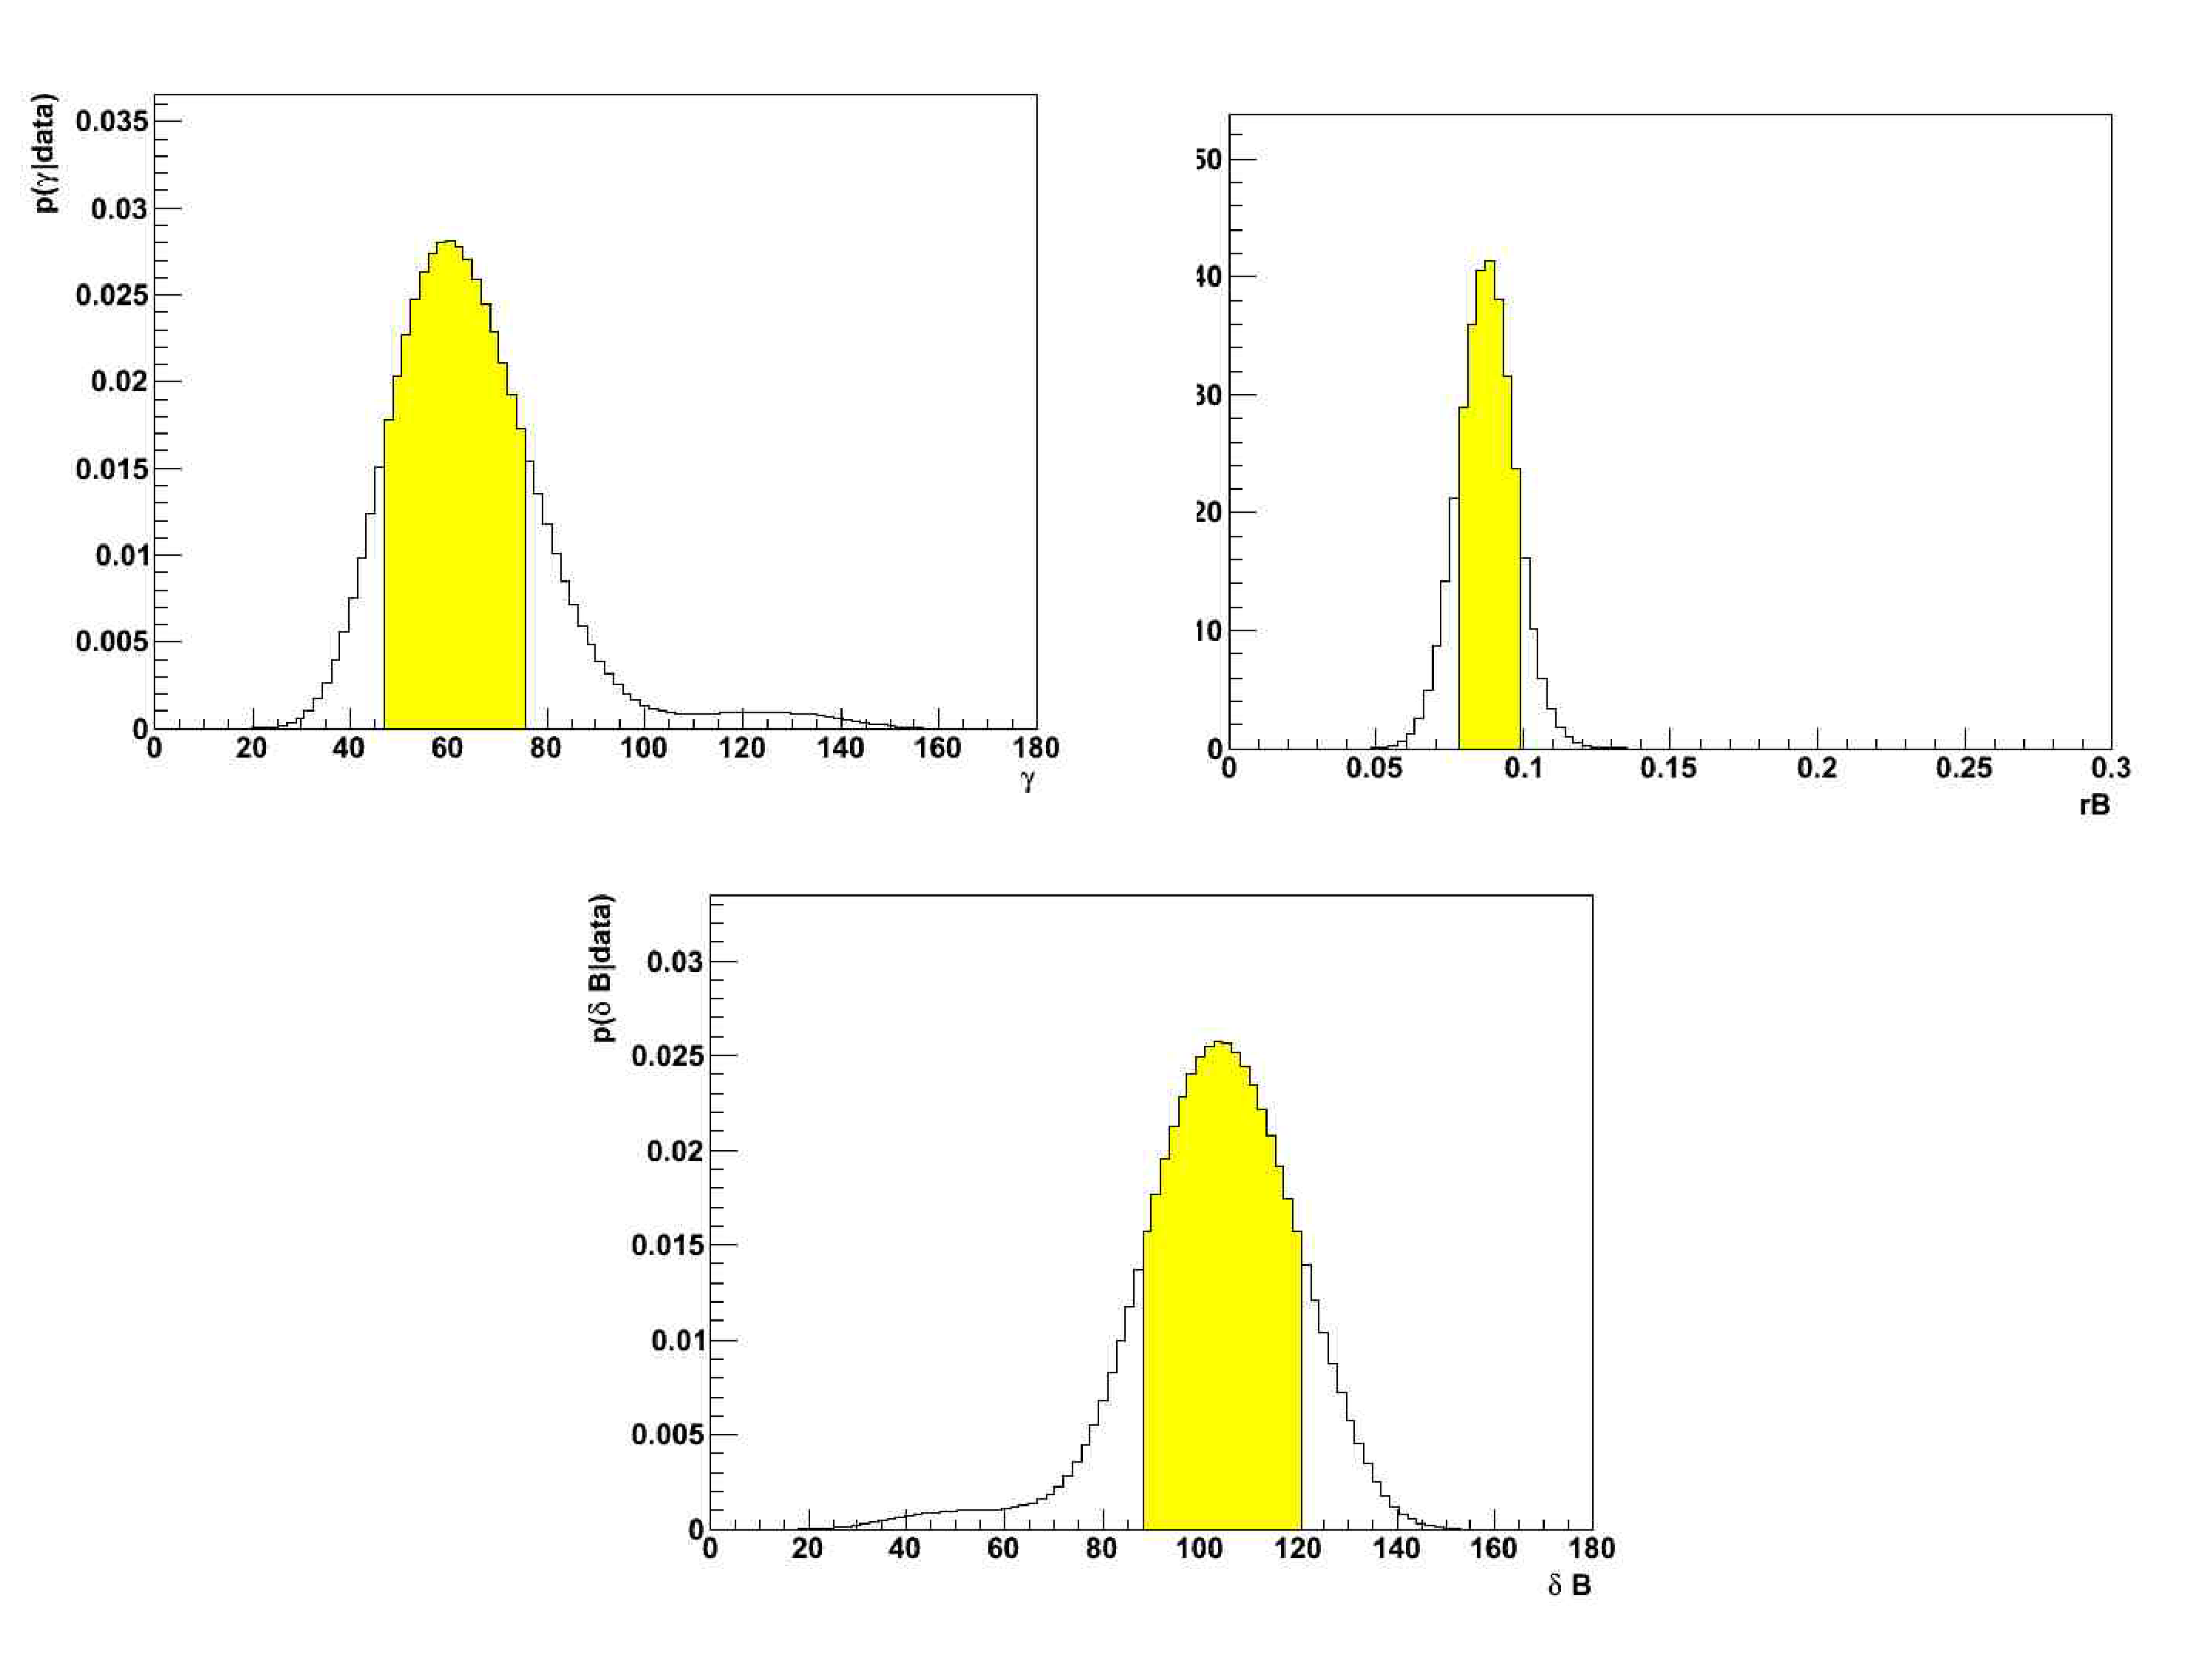
\includegraphics[width=1\textwidth]{Immagini/Plot}
\caption{Distribuzioni di probabilità \emph{a posteriori} di $\gamma$ (in alto a sinistra), $r_B$ (in alto a destra) e $\delta_B$ (in basso). L'area evidenziata in giallo rappresenta il più piccolo intevallo con la più alta densità di probabilità corrispondente al $68\%$ dell'area totale. }
\label{grafici}
\end{center}
\end{figure}

\begin{figure}[htbp] 
\begin{center}
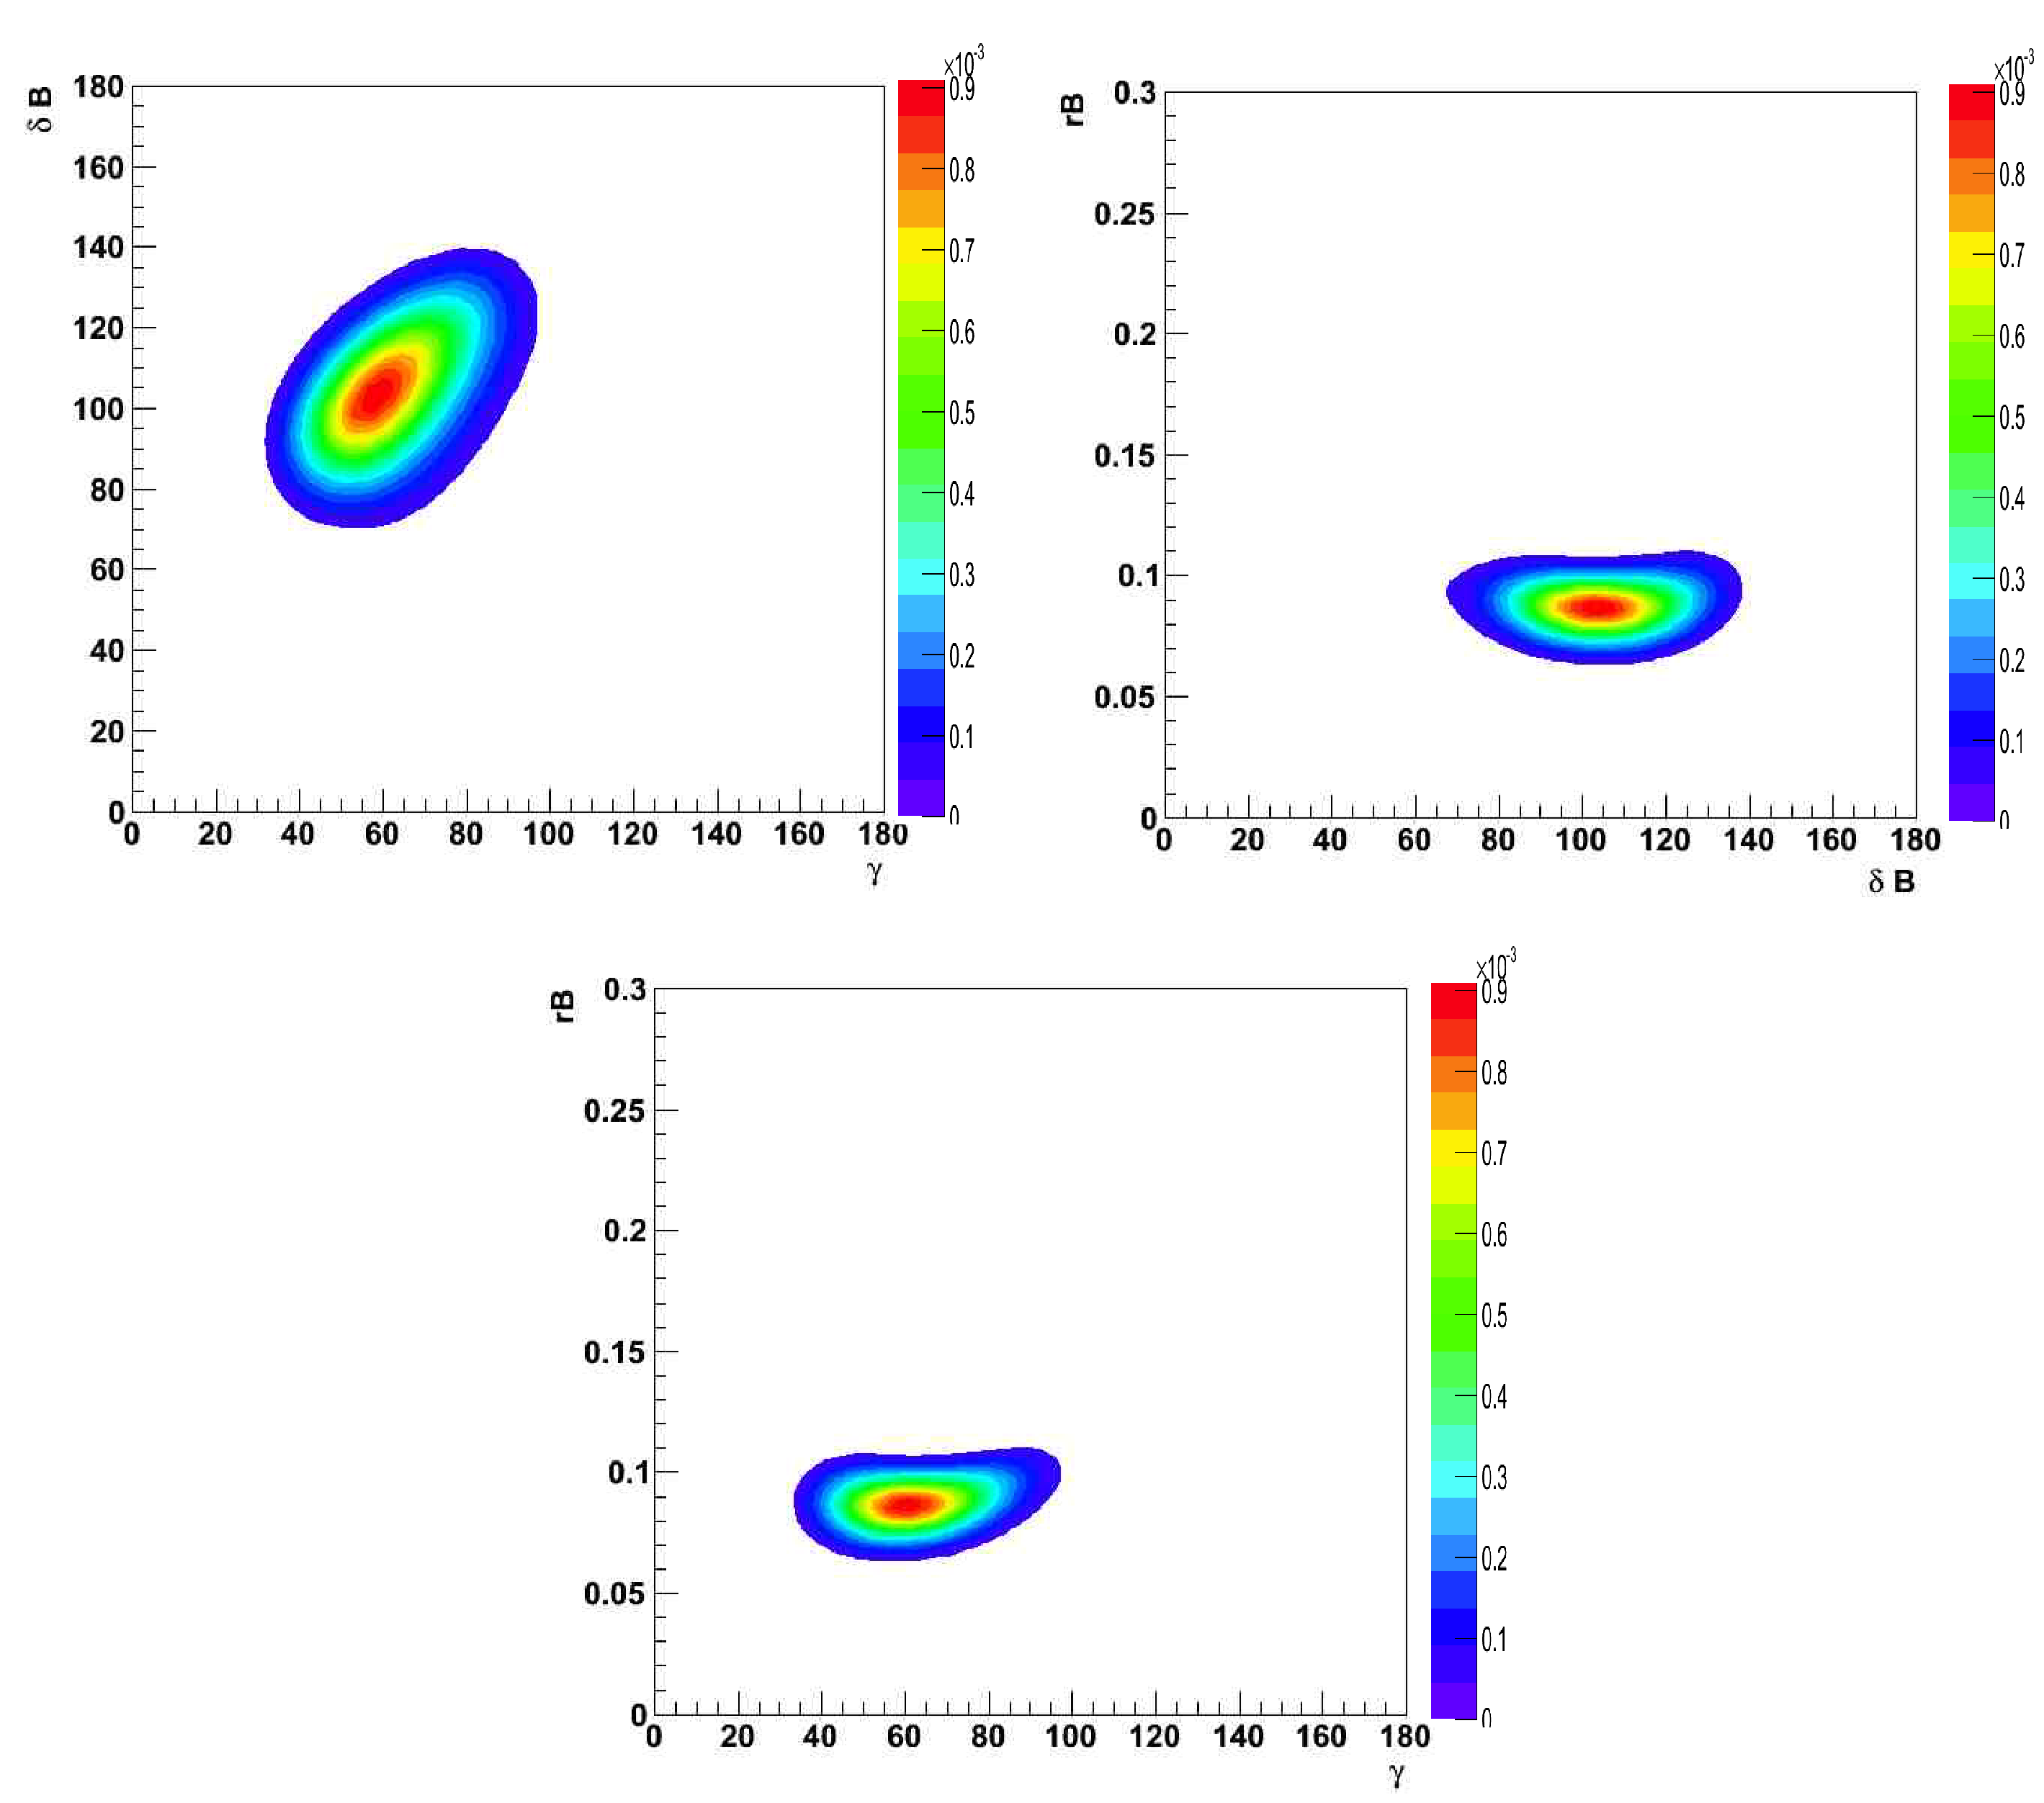
\includegraphics[width=1\textwidth]{Immagini/correlazione}
\caption{Distribuzioni \emph{a posteriori} bidimensionali delle coppie di grandezze $(\gamma, \delta_B)$ (in alto a sinistra), $(\delta_B, r_B)$(in alto a destra) e $(\gamma, r_B)$ (in basso).}
\label{correlazione}
\end{center}
\end{figure}



